% set home directory
\providecommand{\homedir}{..} 
% load the preamble of main.tex by subfiles
\documentclass[\homedir/main.tex]{subfiles}
% ##############################################################################
\begin{document}
% set chapter numbering to work correctly even when separate compilation using subfile
\setcounter{chapter}{0}
\chapter{序論}\label{chap:introduction}

\section{研究背景}\label{sec:background}
現代では,我々はしばしば色やエフェクトなどによって飾り付けられた文字を目にする.
このように装飾された文字は「デザイン文字」と呼ばれる.
デザイン文字は装飾のないシンプルな文字と比べ,目立ちやすく具体的なイメージを与えやすい点で優れている.
例えば,次の\cref{fig:design_char_eg}は赤い「炎」という文字に燃えているようなエフェクトを付与したものであるが,
装飾のない「炎」に比べメラメラと炎が燃えている印象が相手に良く伝わると考えられる.

\begin{figure}[h]
    \centering
    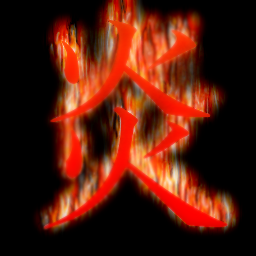
\includegraphics[keepaspectratio, scale=1.0]{design_character_example.png}
    \caption{デザイン文字の例}
    \label{fig:design_char_eg}
\end{figure}

そのため,デザイン文字は特に目立たせたい場合や印象づけたい場合に用いられている.
特に,作品のタイトル・企業名・商品名などのロゴは,印象に残ることが重要なためデザイン文字が用いられることが多い.
しかし,そうしたデザイン文字の作成には高度な技術や多大な時間を要することも多い.
ゆえに,デザイン文字の作成法には研究の意義がある.

\section{研究目的}\label{sec:objective}
本研究では,「デザイン文字列\footnote{デザイン文字の列,すなわち色やエフェクトなどで飾りつけられた文字列のこと}を
別のデザイン文字や文字列画像をもとに自動で生成すること」を目的とする.

\section{本論文の構成}\label{sec:structure}
本論文の構成は,次のようになっている.
\cref{chap:introduction}では,本研究の背景と目的について述べた.
\cref{chap:related_works}では,本研究に関連する先行研究について述べる.
\cref{chap:theories}では,本研究の前提知識となる理論について述べる.
\cref{chap:methods}では,本研究が提案する手法について述べる.
\cref{chap:results}では,実験内容とその結果について述べる.
最後に,\cref{chap:summary}では本論文の結論と今後の課題を述べる.

\printBibForSubfiles
\end{document}